\documentclass[10pt, pdfmx,hiresbb]{beamer}
\usetheme{metropolis}
\usepackage{natbib}
\usepackage{bbm}
\usepackage[utf8]{inputenc}
\usepackage{amsmath}
\usepackage{amsfonts}
\usepackage{amssymb}
\usepackage{amsthm}
\usepackage{textcomp}
\usepackage{gensymb}
\usepackage{appendixnumberbeamer}
\usepackage{siunitx}
\usepackage{lipsum}
\usepackage{float}
\usepackage{pdflscape}
\usepackage{indentfirst}
\usepackage{longtable}
\usepackage{multicol}
\usepackage{makecell}
\usepackage{booktabs}
\usepackage{threeparttable}
\usepackage{graphicx}
\usepackage{setspace} 

\usepackage{color}  % https://dkumor.com/posts/technical/2018/08/15/causal-tikz/
\usepackage{tikz}
\usetikzlibrary{shapes,decorations,arrows,calc,arrows.meta,fit,positioning}
\tikzset{
    -Latex,auto,node distance =1 cm and 1 cm,semithick,
    state/.style ={ellipse, draw, minimum width = 0.7 cm},
    point/.style = {circle, draw, inner sep=0.04cm,fill,node contents={}},
    bidirected/.style={Latex-Latex,dashed},
    el/.style = {inner sep=2pt, align=left, sloped}
}

\newtheorem{prop}{Proposition} 
\setbeamertemplate{thorems}[numbered]

\setbeamerfont{page number in head/foot}{size=\scriptsize}
\setbeamertemplate{footline}[frame number]

\newcommand{\indep}{\rotatebox[origin=c]{90}{$\models$}}

\newcommand\Wider[2][3em]{
\makebox[\linewidth][c]{
  \begin{minipage}{\dimexpr\textwidth+#1\relax}
  \raggedright#2
  \end{minipage}
  }
}

%\usetheme{CambridgeUS}
\setbeamertemplate{navigation symbols}{}
\title[Temperature and Exam]{Winter weather on exam date and matriculation for a prestigious university in Japan}
\author[Suzuki]{Mizuhiro Suzuki}
\date{May 13th, 2021}

\begin{document}
\begin{frame}
\titlepage
\end{frame}

\begin{frame}\frametitle{Research Question \& Roadmap}
  \begin{itemize}
    \item Research Question: Does cold weather on the exam date worsen performance in a high-stakes exam?
    \item Roadmap:
      \begin{itemize}
        \item Background
        \item Data
        \item Empirical strategy
        \item Results
        \item (Some more results not in the paper for now)
      \end{itemize}
    \item A quick heads-up\dots
      \begin{itemize}
        \item Planning to submit the paper to JEEM short 
        \item Max 3,000 words (but ``modestly longer papers will be considered'')
        \item My paper now has 3,200 words
      \end{itemize}
  \end{itemize}
\end{frame}

\begin{frame}\frametitle{Background - Center Test}
  \begin{itemize}
    \item In Japan, for public university admission, students need to take two exams
    \item First-stage: \textcolor{red}{Center Test}
      \begin{itemize}
        \item Held in mid-January (Saturday and Sunday)
          \begin{itemize}
            \item Social science, Japanese, and English on the first day (9:30 AM - 6:10 PM)
            \item Mathematics and natural science on the second day (9:30 AM - 5:50 PM)
          \end{itemize}
        \item Questions are multiple-choice and common for all exam takers
        \item Students take the exam in their own prefectures
      \end{itemize}
    \item Second-stage: University-specific exams
      \begin{itemize}
        \item Public universities hold exams typically in \textcolor{red}{late February} and/or mid-March
        \item Students take the exams at universities they apply for
      \end{itemize}
  \end{itemize}
\end{frame}

\begin{frame}\frametitle{Background - Admission for the University of Tokyo}
  \begin{itemize}
    \item The University of Tokyo (UTokyo) is the most prestigious university in Japan
      \begin{itemize}
        \item Highest-ranked univ. in Japan (73rd ranked in the world ranking) (U.S. News) \\
          (The second highest-ranked univ. is Kyoto University, 125th ranked in the world ranking)
        \item Kawaguchi and Ma (2008): ``The University of Tokyo has occupied the top position of the single-peaked university hierarchy since its establishment in 1877.''
      \end{itemize}
    \item Center Test scores for admission to UTokyo:
      \begin{itemize}
        \item Used for eligibility to take the second-stage exam
          %Thresholds varying across years and majors are set, and if scores at Center Test are below the thresholds, the students cannot take the second-stage exam.
        \item Taken into consideration for final admission 
          \begin{itemize}
            \item The final score of a student is the weighted sum of exam scores at the first- (20\%) and second-stage (80\%) exams
          \end{itemize}
      \end{itemize}
  \end{itemize}
\end{frame}

%\begin{frame}\frametitle{Background - Winter weather and exam performance}
%  \begin{itemize}
%    \item 
%  \end{itemize}
%\end{frame}

\begin{frame}\frametitle{Data}
  \begin{itemize}
    \item Weather information from Japan Meteorological Agency
      \begin{itemize}
        \item Hourly information on temperature, rainfall, snowfall, snow on the ground
        \item I use average between 6 AM to 6 PM
      \end{itemize}
    \item Matriculation for UTokyo from University Basic Information
      \begin{itemize}
        \item Information from 2012 to 2020 on the number of matriculated students for each university by prefectures at which their high schools are located
          \begin{itemize}
            \item By gender (male vs. female)
            \item By major (humanity vs. science)
          \end{itemize}
        \item I calculate the matriculation shares for UTokyo from a prefecture $j$ in year $t$ as 
          \begin{equation*}
            \frac{\text{\# matriculations for UTokyo from $j$ in year $t$}}{\text{\# total matriculations for UTokyo in year $t$}}
          \end{equation*}
      \end{itemize}
  \end{itemize}
\end{frame}

\begin{frame}\frametitle{Summary Statistics}
  \begin{center}
    \begin{table}
      \caption{Summary Statistics}
      \footnotesize
      
\begin{tabular}[t]{lllllll}
\toprule
\multicolumn{1}{c}{ } & \multicolumn{1}{c}{N} & \multicolumn{1}{c}{Mean} & \multicolumn{1}{c}{SD} & \multicolumn{1}{c}{Median} & \multicolumn{1}{c}{Min} & \multicolumn{1}{c}{Max} \\
\cmidrule(l{3pt}r{3pt}){2-2} \cmidrule(l{3pt}r{3pt}){3-3} \cmidrule(l{3pt}r{3pt}){4-4} \cmidrule(l{3pt}r{3pt}){5-5} \cmidrule(l{3pt}r{3pt}){6-6} \cmidrule(l{3pt}r{3pt}){7-7}
Matriculation share (\%) & 423 & 2.08 & 5.23 & 0.79 & 0.06 & 37.35\\
Temperature (\degree C) & 423 & 4.67 & 3.81 & 4.98 & -6.63 & 19.86\\
Hourly precipitation (mm) & 423 & 0.08 & 0.18 & 0.00 & 0.00 & 1.27\\
Hourly snowfall (m) & 423 & 0.00 & 0.00 & 0.00 & 0.00 & 0.01\\
Cumulated snow (m) & 423 & 0.05 & 0.15 & 0.00 & 0.00 & 1.26\\
\bottomrule
\end{tabular}

      \tiny
      \begin{tablenotes}
        \item 
          Notes:
          Matriculation share (\%) is the share of newly matriculated students to the University of Tokyo from each prefecture.
          The matriculation share is calculated based on the ratio of the number of students from high schools in the prefecture to the total number of matriculation.
          I use weather variables at prefecture capitals between 6 AM and 6 PM on days of Center Test.
      \end{tablenotes}
    \end{table}
  \end{center}
\end{frame}

\begin{frame}\frametitle{Map of matriculation shares (\%)}
  \begin{center}
    \begin{figure}
      %\caption{Map of matriculation shares (\%)}
      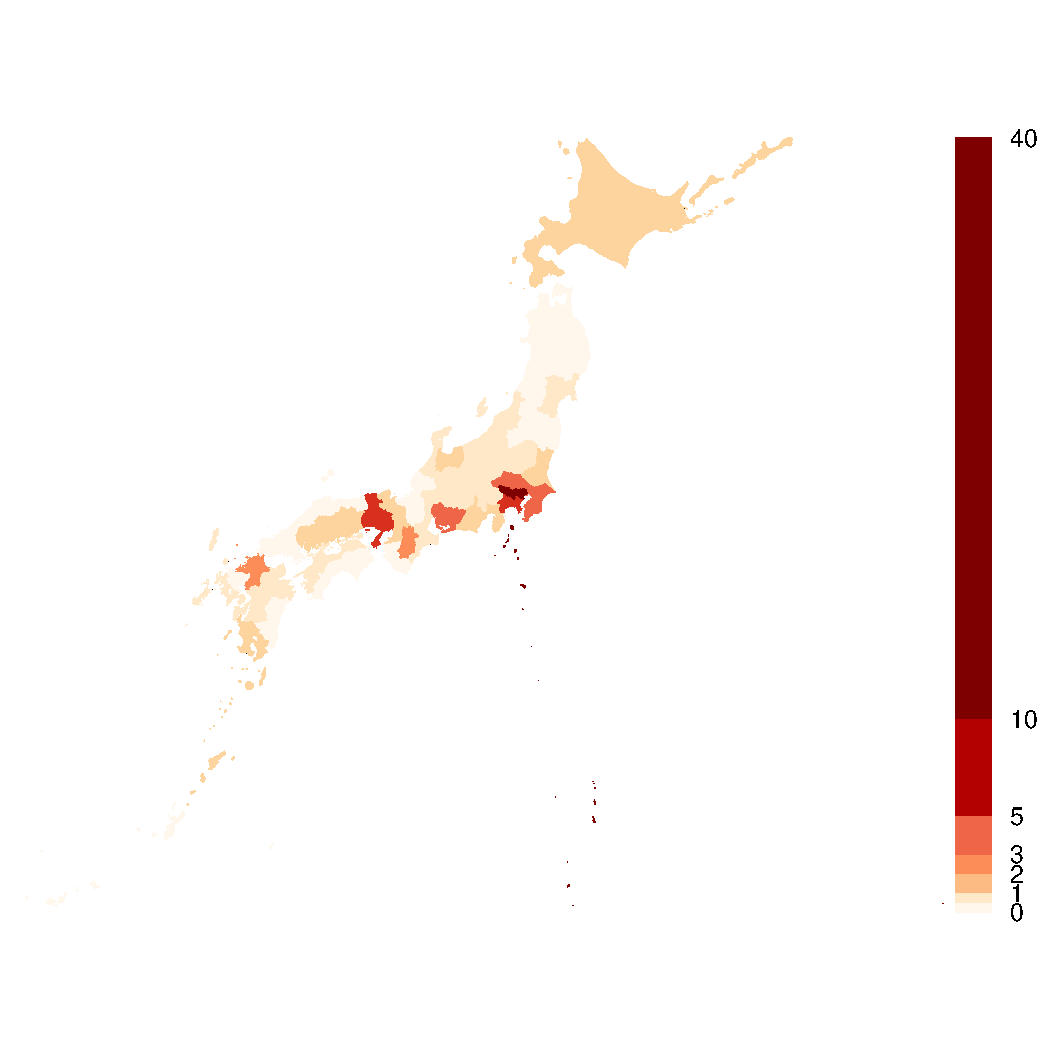
\includegraphics[width=7cm]{../Output/images/admission_map.pdf}
      \tiny
      \begin{tablenotes}
      \item Notes:
        This map shows the matriculation shares (\%) for the University of Tokyo from each prefecture.
        The matriculation share is calculated based on the ratio of the number of students from high schools in the prefecture to the total number of matriculation.
        Average of the shares across years is shown in the map.
        Although not shown in the legend due to the lack of the space, the lightest color in the map means the matriculation share between 0 to 0.5\% 
        The darkest prefecture in the east part of Japan is Tokyo.
      \end{tablenotes}
    \end{figure}
  \end{center}
\end{frame}

\begin{frame}\frametitle{Empirical Strategy - Why UTokyo?}
  \begin{itemize}
    \item Suppose that low temperature negatively affects exam performance
    \item If I consider a matriculation for a middle-ranked university,
      \begin{enumerate}
        \item students in the prefecture who would have gotten into the middle-ranked university if the temperature were higher may end up in a lower-ranked university instead, but
        \item students in the prefecture who would have gotten into a higher-ranked university may end up in the middle-ranked university instead
      \end{enumerate}
    \item Considering matriculation for UTokyo (the most prestigious university in Japan) rules out the second possibility
  \end{itemize}
\end{frame}

\begin{frame}\frametitle{Empirical Strategy - Estimation equation}
  \label{est_eq}
  \begin{equation*}
    Y_{jt} = \sum_k \alpha_k T_{jt}^k + X_{jt}' \beta + \mu_j + \tau_t + \epsilon_{jt}.
  \end{equation*}
  \begin{itemize}
    \item $Y_{jt}$: matriculation share (\%) for UTokyo of a prefecture $j$ in year $t$
    \item $T_{jt}^k$: $k$'th temperature interval 
      \begin{itemize}
        \item 3-$\degree$C intervals
        \item Average across two exam dates in $j$ in year $t$
      \end{itemize}
    \item $X_{jt}$: other weather variables such as rainfall, snowfall, and cumulated snow on the ground on exam date
    \item $\mu_j$: prefecture fixed effects
    \item $\tau_t$: year fixed effects
    \item $\epsilon_{jt}$: error term
    \item Standard errors are clustered at the prefecture level 
  \end{itemize}
  \hyperlink{temp_dev_1}{\beamergotobutton{Temperature variation}}
  \hyperlink{temp_dev_2}{\beamergotobutton{Within-prefecture temperature variation}}
\end{frame}

\begin{frame}\frametitle{Temperature effects on the matriculation shares (\%) \\ {\small Low temperature negatively affects exam performance}}
  \begin{center}
    \begin{figure}
      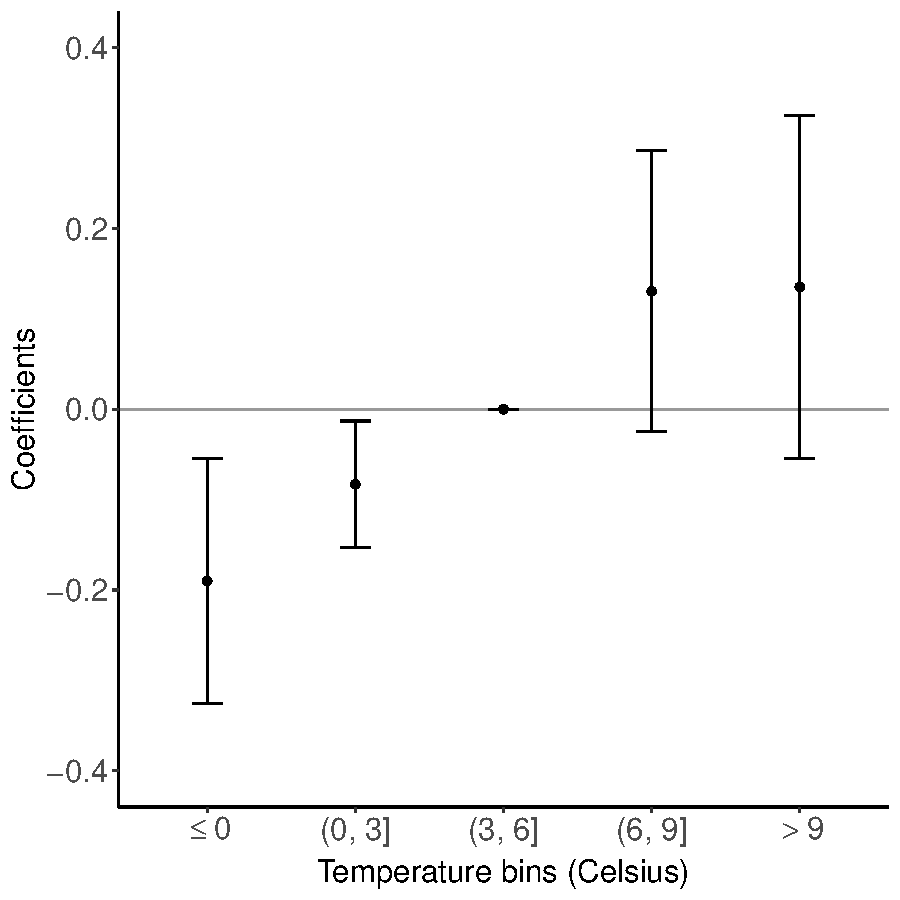
\includegraphics[width=6.5cm]{../Output/images/main_reg_2.pdf}
      \tiny
      \begin{tablenotes}
      \item Notes:
        The figure shows the regression coefficients of the matriculation shares for UTokyo (\%) on temperature bins.
        I use temperature at prefecture capitals between 6 AM and 6 PM on days of Center Test.
        The 90\% confidence intervals are shown.
        Prefecture fixed effects and year fixed effects are also included.
        Standard errors are clustered at the prefecture level.
      \end{tablenotes}
    \end{figure}
  \end{center}
\end{frame}

\begin{frame}\frametitle{{\normalsize Effects of other weather variables on the matriculation shares (\%)} \\ {\small Cumulated snow on the ground negatively affects exam performance}}
    \begin{table}[h]
      \Wider[4em]{
      \center
      \fontsize{6}{7}\selectfont
      
% Table created by stargazer v.5.2.2 by Marek Hlavac, Harvard University. E-mail: hlavac at fas.harvard.edu
% Date and time: Tue, May 04, 2021 - 11:24:34
\begin{tabular}{@{\extracolsep{5pt}}lccc} 
\\[-1.8ex]\hline 
\hline \\[-1.8ex] 
 & \multicolumn{3}{c}{\textit{Dependent variable:}} \\ 
\cline{2-4} 
\\[-1.8ex] & \multicolumn{3}{c}{Matriculation share (\%)} \\ 
\\[-1.8ex] & (1) & (2) & (3)\\ 
\hline \\[-1.8ex] 
 Rainfall (mm) & $-$0.02 & 0.06 & 0.06 \\ 
  & (0.09) & (0.08) & (0.08) \\ 
  & & & \\ 
 Snowfall (m) & 7.75 &  &  \\ 
  & (9.95) &  &  \\ 
  & & & \\ 
 Cumulated snow (m) &  & $-$0.19$^{**}$ &  \\ 
  &  & (0.09) &  \\ 
  & & & \\ 
 Cumulated snow $>$ .10 m &  &  & $-$0.11$^{***}$ \\ 
  &  &  & (0.04) \\ 
  & & & \\ 
\hline \\[-1.8ex] 
Temperature bins & Yes & Yes & Yes \\ 
Prefecture FE & Yes & Yes & Yes \\ 
Year FE & Yes & Yes & Yes \\ 
Observations & 423 & 423 & 423 \\ 
\hline 
\hline \\[-1.8ex] 
\textit{Note:}  & \multicolumn{3}{r}{$^{*}$p$<$0.1; $^{**}$p$<$0.05; $^{***}$p$<$0.01} \\ 
\end{tabular} 

      \tiny
      \begin{tablenotes}
      \item 
        The outcome variable is the matriculation shares (\%) for the University of Tokyo from each prefecture.
        The matriculation share is calculated based on the ratio of the number of students from high schools in the prefecture to the total number of matriculation.
        I use weather variables at prefecture capitals between 6 AM and 6 PM on days of Center Test.
        Standard errors are clustered at the prefecture level.
      \end{tablenotes}
    }
    \end{table}
\end{frame}

\begin{frame}\frametitle{Placebo test (including temperature one year after the exams)}
  \begin{figure}
    \begin{minipage}{0.49\textwidth}
      \begin{center}
        Contemporaneous temperature
      \end{center}
      \begin{figure}[h]
        \centering
        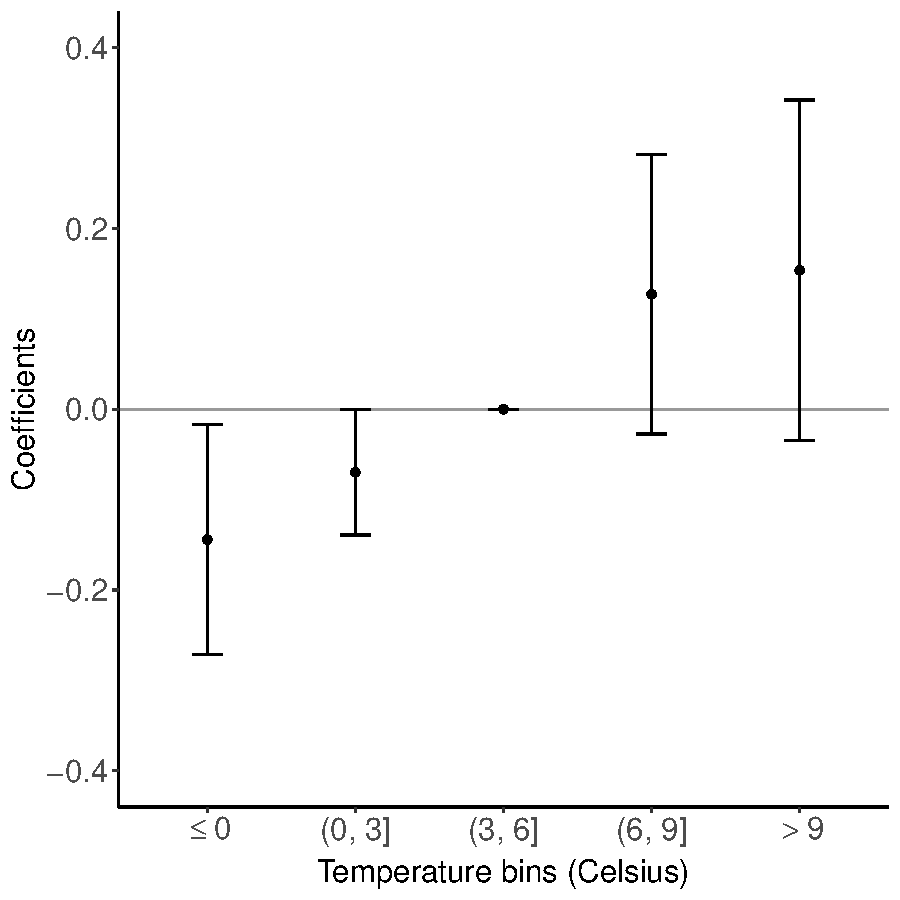
\includegraphics[width = \textwidth]{../Output/images/reg_placebo_exam_4.pdf}
      \end{figure}
    \end{minipage}
    \begin{minipage}{0.49\textwidth}
      \begin{center}
        Temperature one year later
      \end{center}
      \begin{figure}[h]
        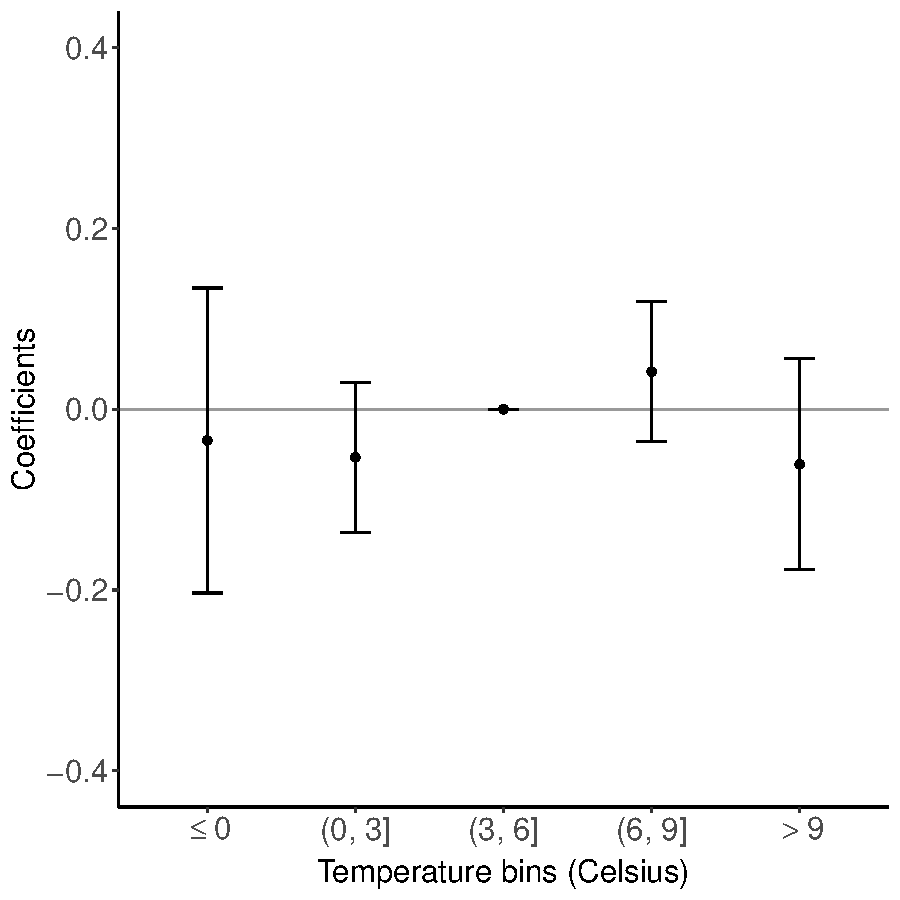
\includegraphics[width = \textwidth]{../Output/images/reg_placebo_f1_4.pdf}
        \centering
      \end{figure}
    \end{minipage}
    \tiny
    \begin{tablenotes}
    \item Notes;
      The figures show the regression coefficients of the matriculation shares for UTokyo (\%) on temperature bins.
      In the left figure, the estimates on the contemporaneous temperature bins are shown.
      In the right figure, the estimates on the temperature one year later are shown.
      Rainfall and cumulated snow on the ground (both contemporaneous and one year later) are included in the regression.
      The 90\% confidence intervals are shown.
      Prefecture fixed effects and year fixed effects are also included.
      Standard errors are clustered at the prefecture level.
    \end{tablenotes}
  \end{figure}
\end{frame}

\begin{frame}\frametitle{Cognitive performance at the exam vs. Preparation \\ {\small Temperature on the exam date matters}}
  \begin{figure}
    \center
    \begin{minipage}{0.43\textwidth}
      \begin{center}
        Temperature on the exam date \smallskip
      \end{center}
      \begin{figure}[h]
        \centering
        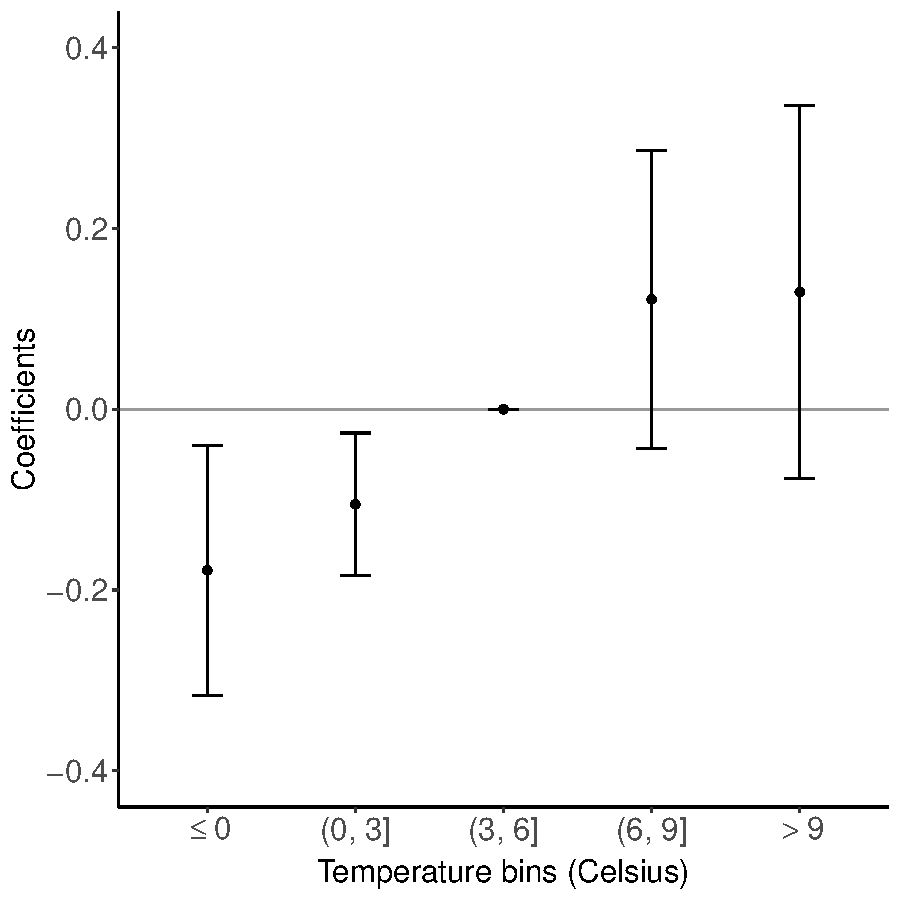
\includegraphics[width = \textwidth]{../Output/images/reg_pre10_exam_4.pdf}
      \end{figure}
    \end{minipage}
    \begin{minipage}{0.43\textwidth}
      \begin{center}
        Average temperature for 10 days before the exam
      \end{center}
      \begin{figure}[h]
        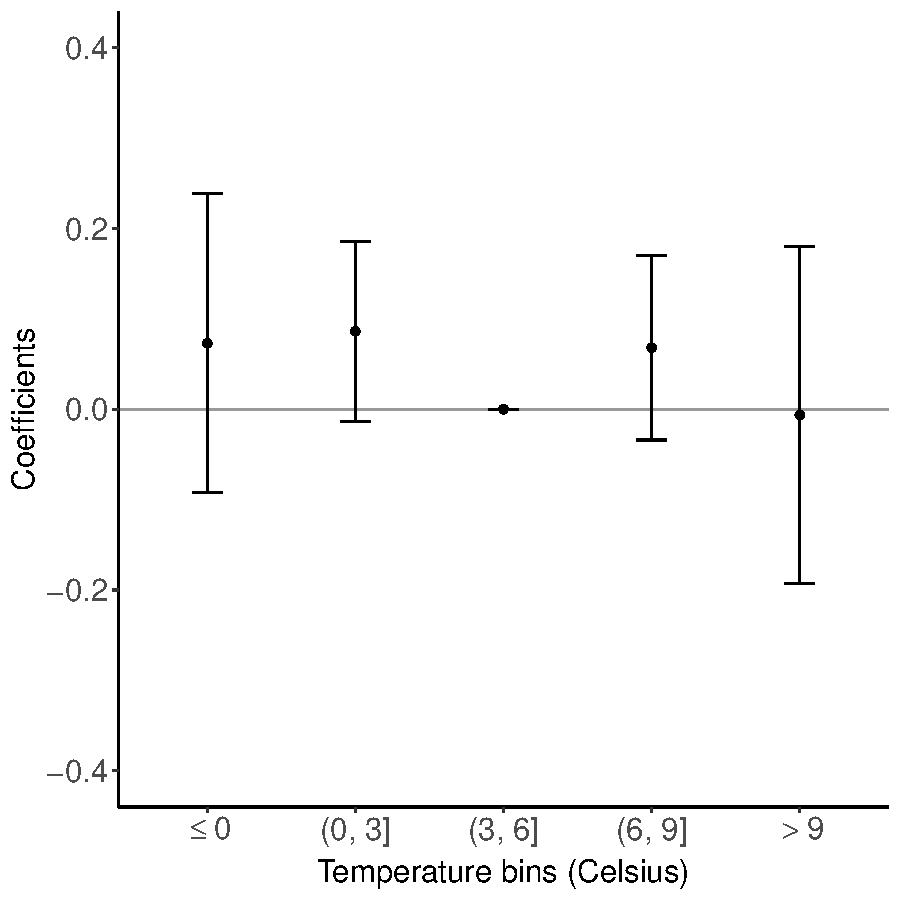
\includegraphics[width = \textwidth]{../Output/images/reg_pre10_pre10_4.pdf}
        \centering
      \end{figure}
    \end{minipage}
    \tiny
    \begin{tablenotes}
    \item Notes;
      The figures show the regression coefficients of the matriculation shares for UTokyo (\%) on temperature bins.
      In the left figure, the estimates on the temperature on the exam date are shown.
      In the right figure, the estimates on the average temperature for 10 days before the exam are shown.
      Rainfall and cumulated snow on the ground (both on the exam days and average for 10 days before the exam) are included in the regression.
      The 90\% confidence intervals are shown.
      Prefecture fixed effects and year fixed effects are also included.
      Standard errors are clustered at the prefecture level.
    \end{tablenotes}
  \end{figure}
\end{frame}

\begin{frame}
  \frametitle{Additional analyses}
  \begin{itemize}
    \item Take population into account for the outcome variable:
      \begin{equation*}
        \frac{\text{\# matriculations for UTokyo from $j$ in year $t$}}{\text{Population (million) in $j$ in year $t$}}
      \end{equation*}
    \item Weather variables
      \begin{itemize}
        \item Average between 6AM and 6PM was used
        \item See the effects of weather between 6AM-9AM (morning) and 9AM-6PM (during exam) separately
      \end{itemize}
    \item Male vs. Female
      \begin{itemize}
        \item Women are more sensitive to temperature changes?
      \end{itemize}
    \item Humanity vs. Science
  \end{itemize}
\end{frame}

\begin{frame}\frametitle{Some additional analysis: Matriculation per population}
  \begin{figure}
    \begin{minipage}{0.44\textwidth}
      \begin{center}
        Matriculation per pop. (total) \\ (mean: 17.3)
      \end{center}
      \begin{figure}[h]
        \centering
        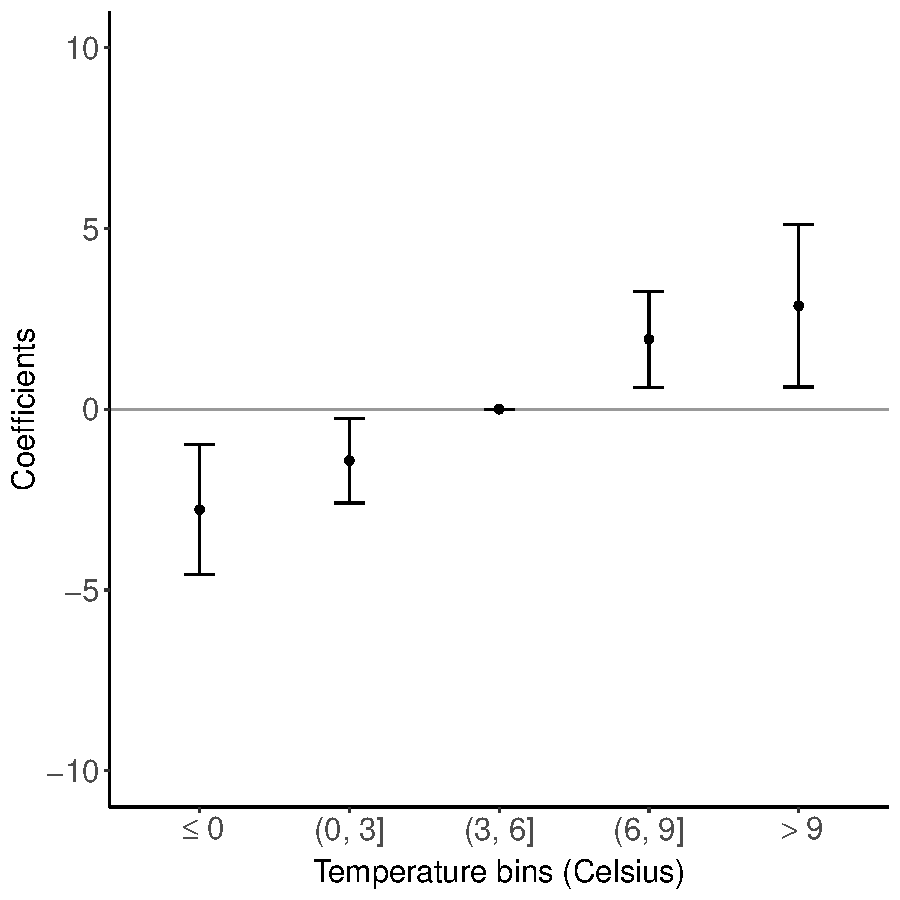
\includegraphics[width = \textwidth]{../Output/images/per_pop_reg_2.pdf}
      \end{figure}
    \end{minipage}
    \begin{minipage}{0.44\textwidth}
      \begin{center}
        Matriculation per pop. (15-19-year-old) (mean: 361)
      \end{center}
      \begin{figure}[h]
        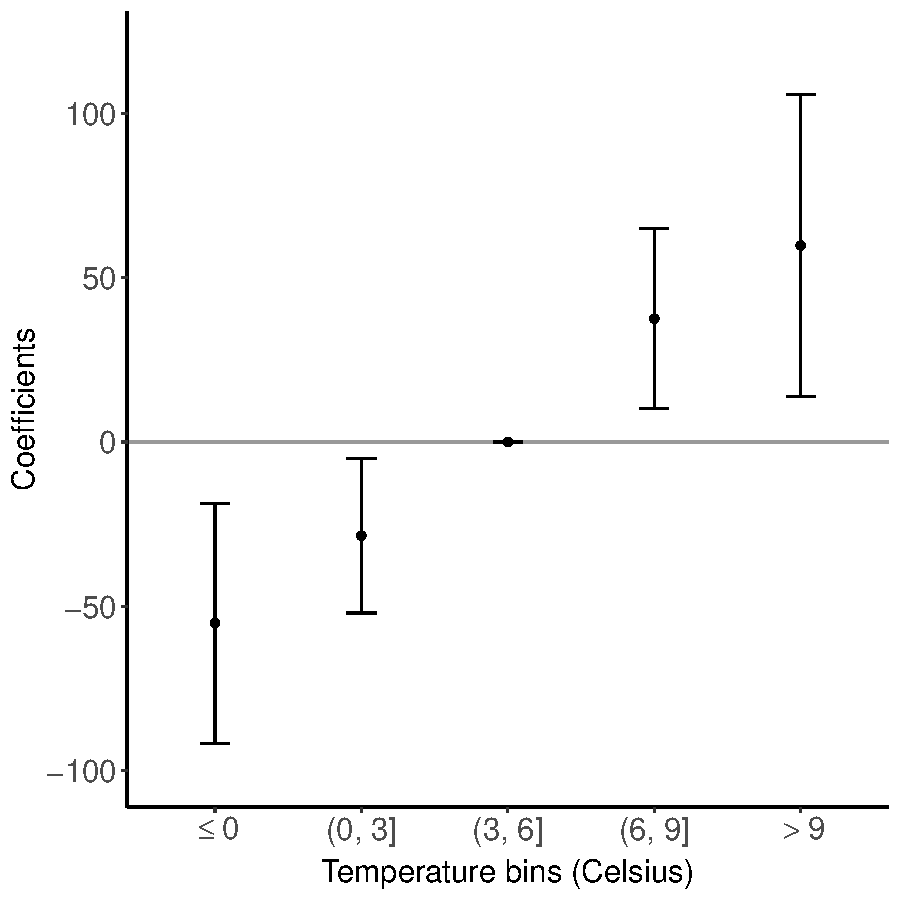
\includegraphics[width = \textwidth]{../Output/images/per_pop_reg_4.pdf}
        \centering
      \end{figure}
    \end{minipage}
    \tiny
    \begin{tablenotes}
    \item Notes;
      The figures show the regression coefficients of the matriculation for UTokyo (\%) per population on temperature bins.
      In the left figure, the matriculation per population (million) is used as an outcome.
      In the right figure, the matriculation per 15-19-year-old population (million) is used as an outcome.
      Rainfall and cumulated snow on the ground on the exam date are included in the regression.
      Prefecture fixed effects and year fixed effects are also included.
      The 90\% confidence intervals are shown.
      Standard errors are clustered at the prefecture level.
    \end{tablenotes}
  \end{figure}
\end{frame}

\begin{frame}\frametitle{Some additional analysis: Matriculation per population \\ Placebo test (oh no!)}
  \begin{figure}
    \begin{minipage}{0.44\textwidth}
      \begin{center}
        Matriculation per pop. (total) \\ (contemporaneous temp.)
      \end{center}
      \begin{figure}[h]
        \centering
        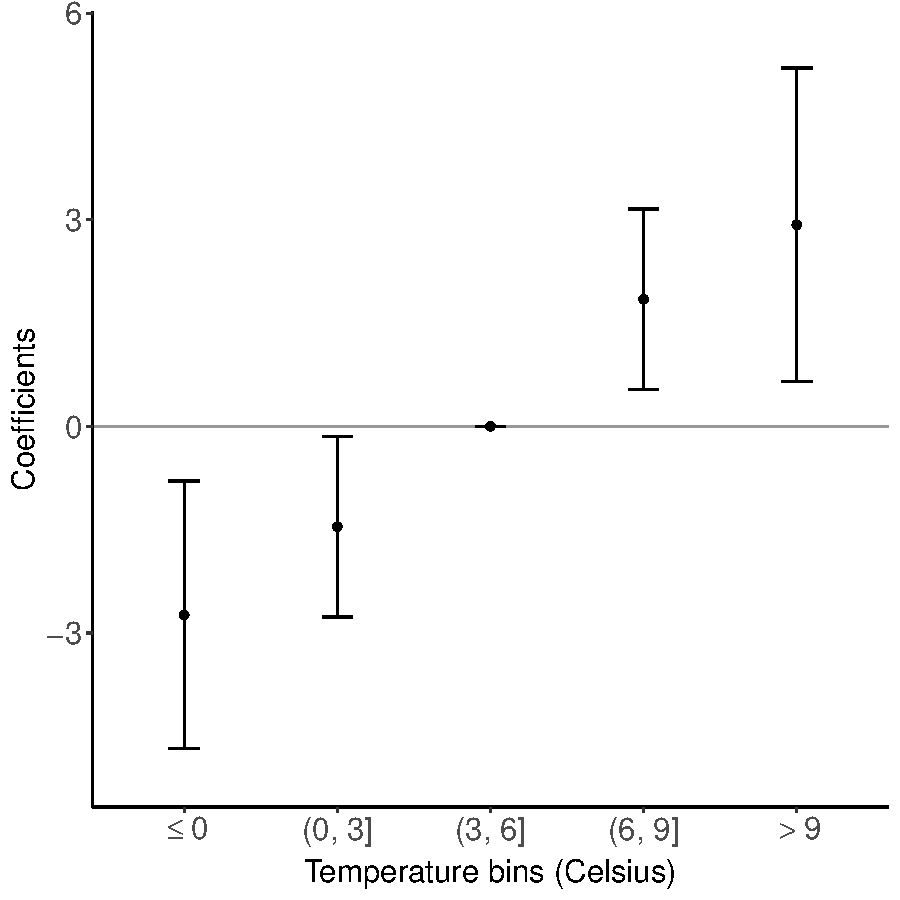
\includegraphics[width = \textwidth]{../Output/images/per_pop_reg_t.pdf}
      \end{figure}
    \end{minipage}
    \begin{minipage}{0.44\textwidth}
      \begin{center}
        Matriculation per pop. (total) (temp. one year after)
      \end{center}
      \begin{figure}[h]
        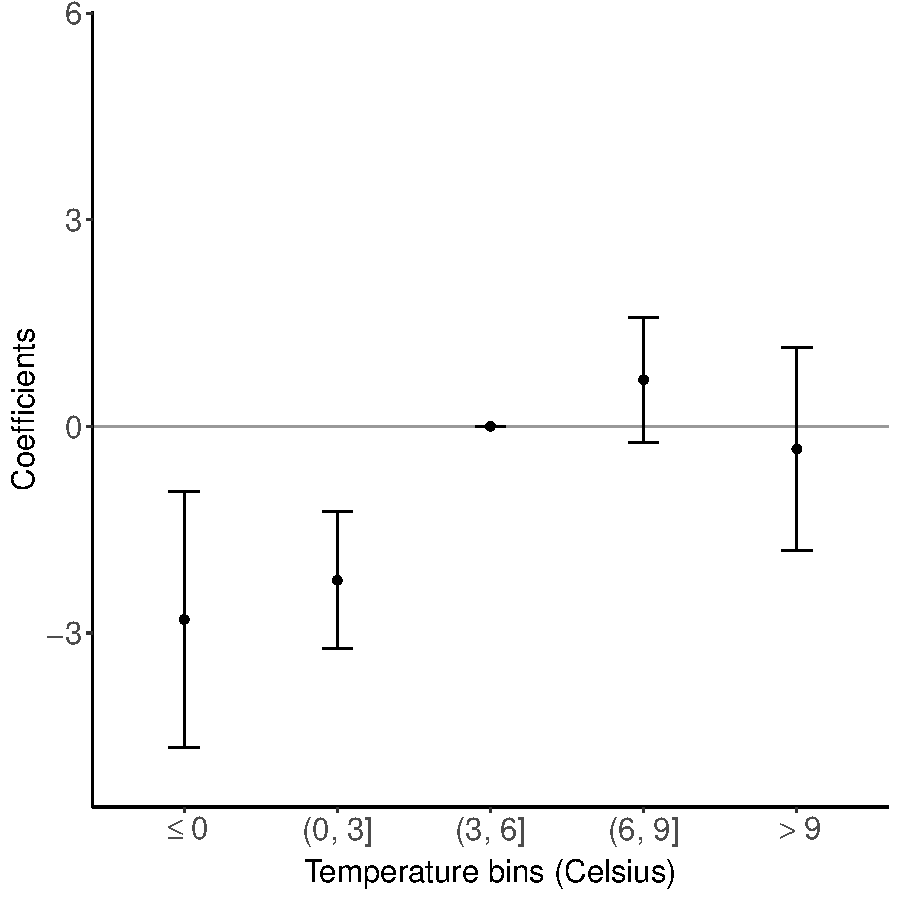
\includegraphics[width = \textwidth]{../Output/images/per_pop_reg_f1.pdf}
        \centering
      \end{figure}
    \end{minipage}
    \tiny
    \begin{tablenotes}
    \item Notes;
      The figures show the regression coefficients of the matriculation for UTokyo (\%) per population (total, million) on temperature bins.
      In the left figure, the estimates on the contemporaneous temperature bins are shown.
      In the right figure, the estimates on the temperature one year later are shown.
      Rainfall and cumulated snow on the ground on the exam date are included in the regression.
      Prefecture fixed effects and year fixed effects are also included.
      The 90\% confidence intervals are shown.
      Standard errors are clustered at the prefecture level.
    \end{tablenotes}
  \end{figure}
\end{frame}

\begin{frame}\frametitle{Some additional analysis: Population \\ Temperature on exam date affects population...?}
  \begin{figure}
    \begin{minipage}{0.44\textwidth}
      \begin{center}
        Total population (million) \\ (contemporaneous temp.)
      \end{center}
      \begin{figure}[h]
        \centering
        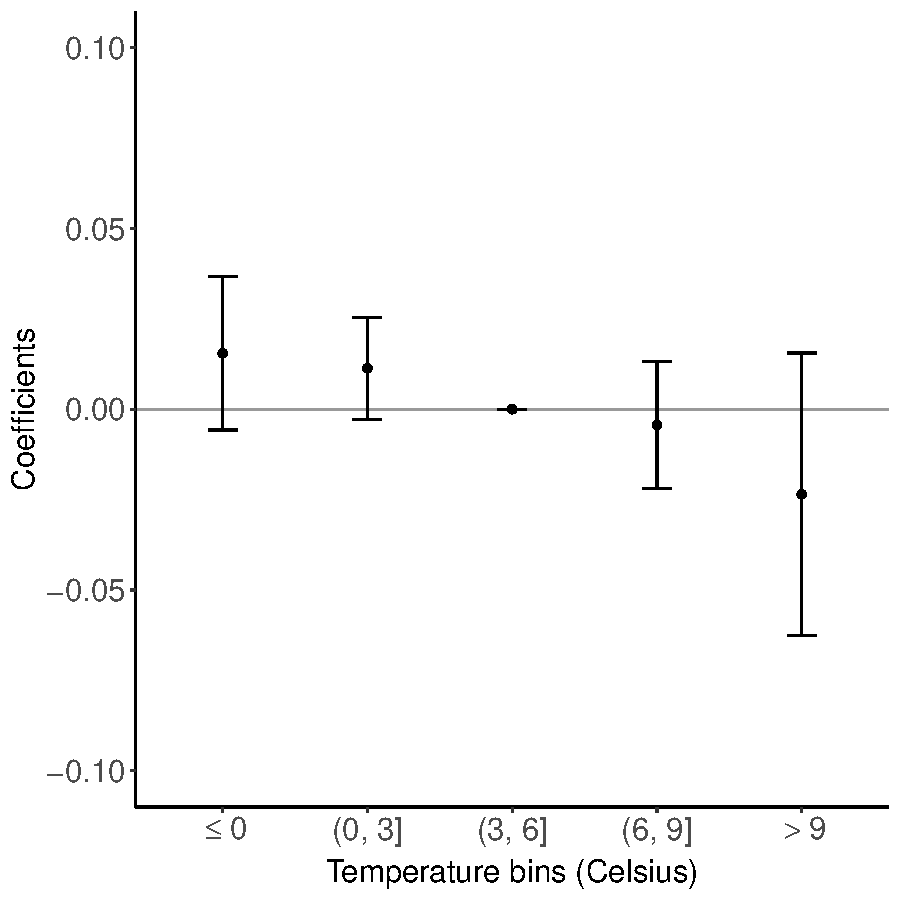
\includegraphics[width = \textwidth]{../Output/images/pop_reg_t.pdf}
      \end{figure}
    \end{minipage}
    \begin{minipage}{0.44\textwidth}
      \begin{center}
        Total population (million) \\ (temp. one year after)
      \end{center}
      \begin{figure}[h]
        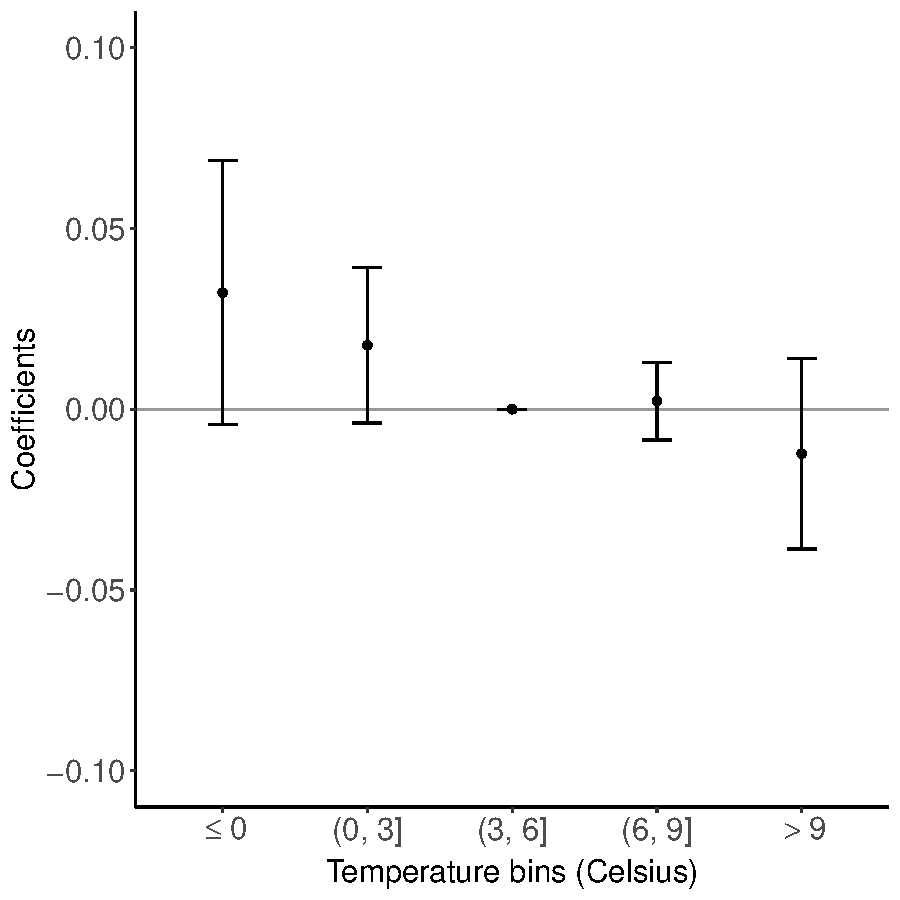
\includegraphics[width = \textwidth]{../Output/images/pop_reg_f1.pdf}
        \centering
      \end{figure}
    \end{minipage}
    \tiny
    \begin{tablenotes}
    \item Notes;
      The figures show the regression coefficients of the population (total, million) on temperature bins.
      In the left figure, the estimates on the contemporaneous temperature bins are shown.
      In the right figure, the estimates on the temperature one year later are shown.
      Rainfall and cumulated snow on the ground on the exam date are included in the regression.
      Prefecture fixed effects and year fixed effects are also included.
      The 90\% confidence intervals are shown.
      Standard errors are clustered at the prefecture level.
    \end{tablenotes}
  \end{figure}
\end{frame}

\begin{frame}\frametitle{{\normalsize Some additional analysis: Temperature in the morning vs. during exam} \\ {\small Temperature in the morning matters more, maybe?}}
  \begin{figure}
    \begin{minipage}{0.44\textwidth}
      \begin{center}
        Temperature in the morning \\ (6AM - 9AM)
      \end{center}
      \begin{figure}[h]
        \centering
        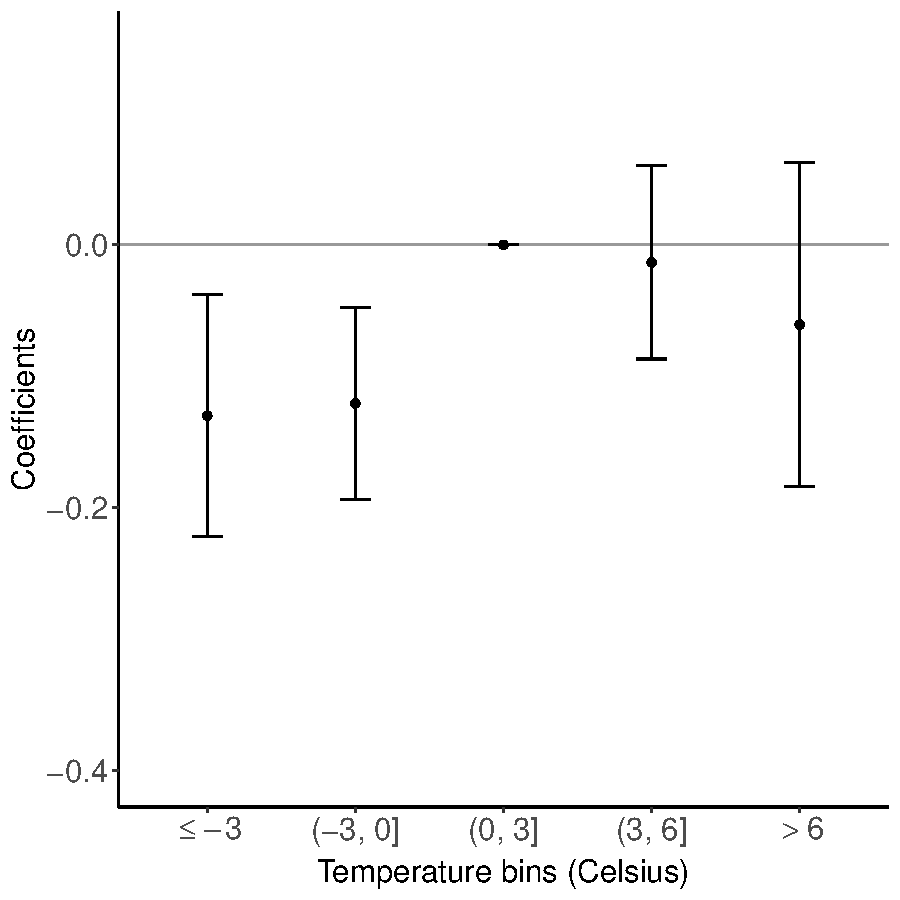
\includegraphics[width = \textwidth]{../Output/images/morning_exam_reg_6_morning.pdf}
      \end{figure}
    \end{minipage}
    \begin{minipage}{0.44\textwidth}
      \begin{center}
        Temperature during exam \\ (9AM - 6PM)
      \end{center}
      \begin{figure}[h]
        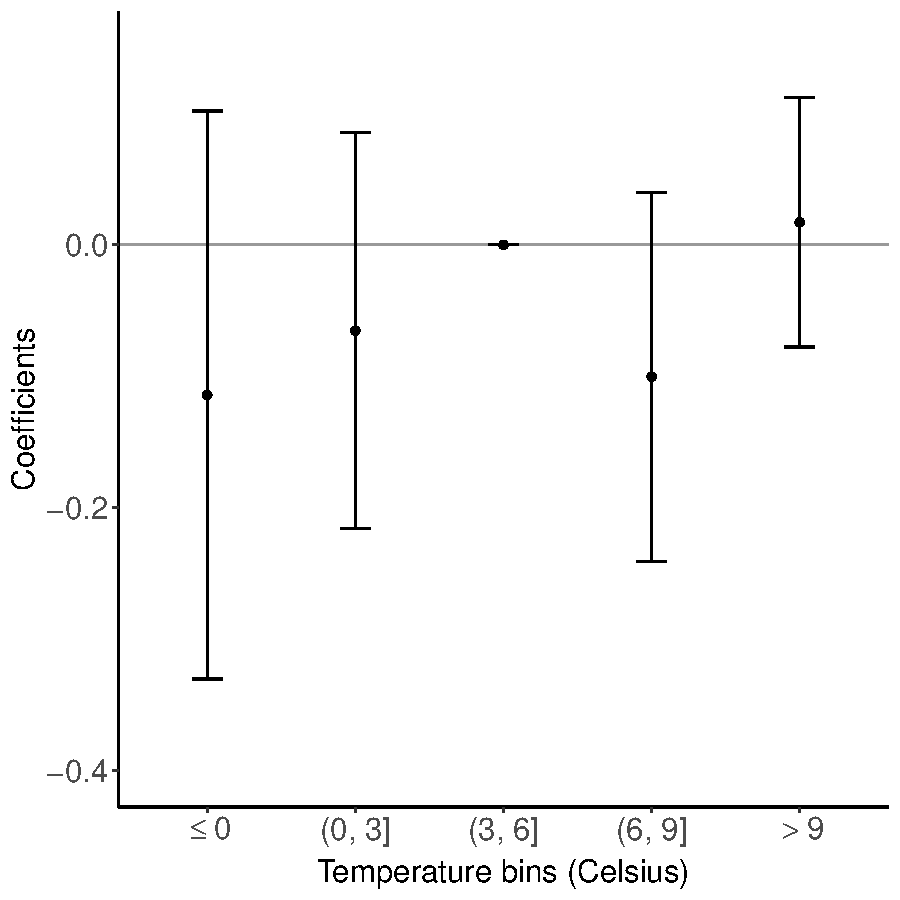
\includegraphics[width = \textwidth]{../Output/images/morning_exam_reg_6_exam.pdf}
        \centering
      \end{figure}
    \end{minipage}
    \tiny
    \begin{tablenotes}
    \item Notes;
      The figures show the regression coefficients of the matriculation shares for UTokyo (\%) on temperature bins.
      In the left figure, the estimates on the temperature (average between 6AM and 9AM) bins are shown.
      In the right figure, the estimates on the temperature (average between 9AM and 6PM) bins are shown.
      Rainfall and cumulated snow on the ground (both in the morning and during exam) are included in the regression.
      The 90\% confidence intervals are shown.
      Prefecture fixed effects and year fixed effects are also included.
      Standard errors are clustered at the prefecture level.
    \end{tablenotes}
  \end{figure}
\end{frame}

\begin{frame}\frametitle{Some additional analysis: Female vs. Male \\ {\small Female students are less affected by temperature\dots or maybe not?}}
  \begin{figure}
    \center
    \begin{minipage}{0.43\textwidth}
      \begin{center}
        Female \\
        {\small (mean: 0.38 \%, median: 0.13 \%)}
      \end{center}
      \begin{figure}[h]
        \centering
        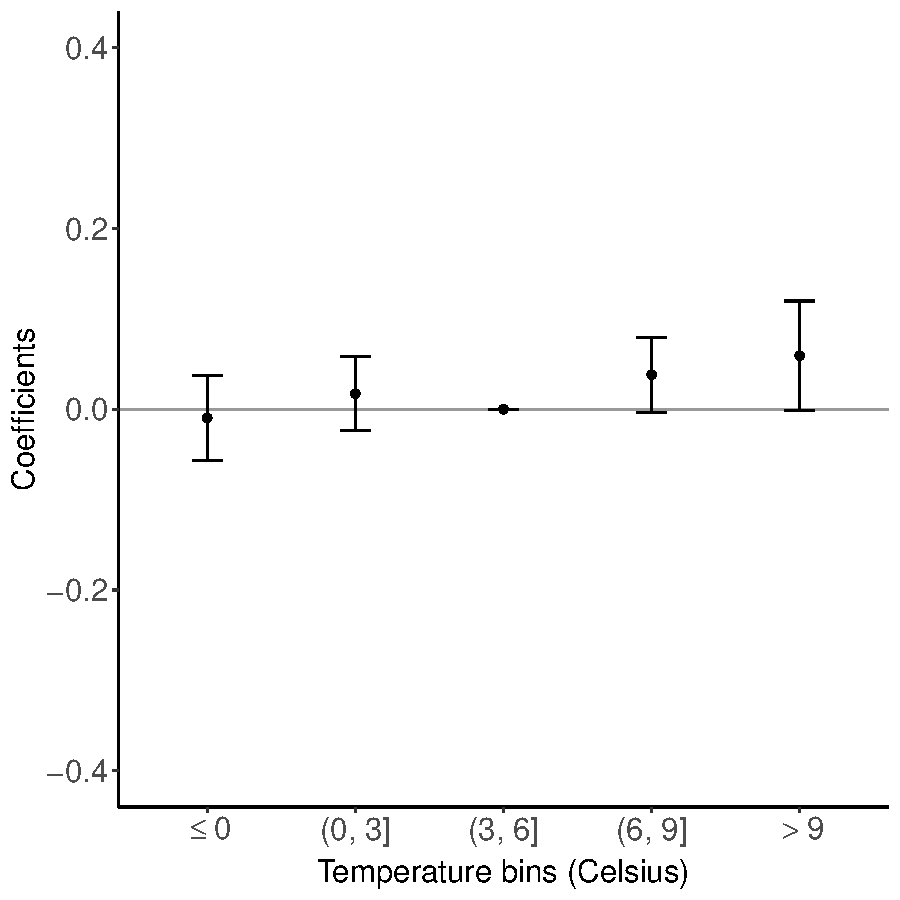
\includegraphics[width = \textwidth]{../Output/images/reg_gender_2.pdf}
      \end{figure}
    \end{minipage}
    \begin{minipage}{0.43\textwidth}
      \begin{center}
        Male \\
        {\small (mean: 1.70 \%, median: 0.61 \%)}
      \end{center}
      \begin{figure}[h]
        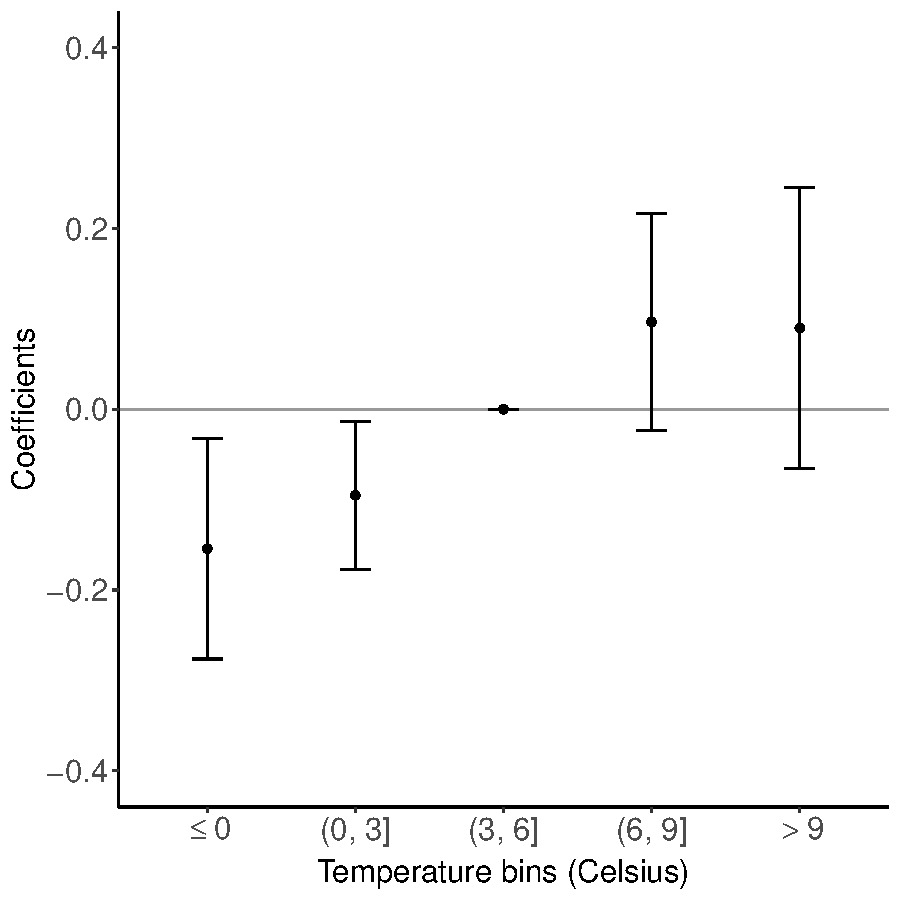
\includegraphics[width = \textwidth]{../Output/images/reg_gender_4.pdf}
        \centering
      \end{figure}
    \end{minipage}
    \tiny
    \begin{tablenotes}
    \item Notes;
      The figures show the regression coefficients of the matriculation shares for UTokyo (\%) on temperature bins.
      In the left figure, the outcome is the matriculation share of female students from each prefecture.
      In the right figure, the outcome is the matriculation share of male students from each prefecture.
      Rainfall and cumulated snow on the ground (both on the exam days and average for 10 days before the exam) are included in the regression.
      The 90\% confidence intervals are shown.
      Prefecture fixed effects and year fixed effects are also included.
      Standard errors are clustered at the prefecture level.
    \end{tablenotes}
  \end{figure}
\end{frame}

\begin{frame}\frametitle{Some additional analysis: Humanity vs. Science \\ {\small No significant difference in temperature effects}}
  \begin{figure}
    \center
    \begin{minipage}{0.43\textwidth}
      \begin{center}
        Humanity \\
        {\small (mean: 2.07 \%, median: 0.76 \%)}
      \end{center}
      \begin{figure}[h]
        \centering
        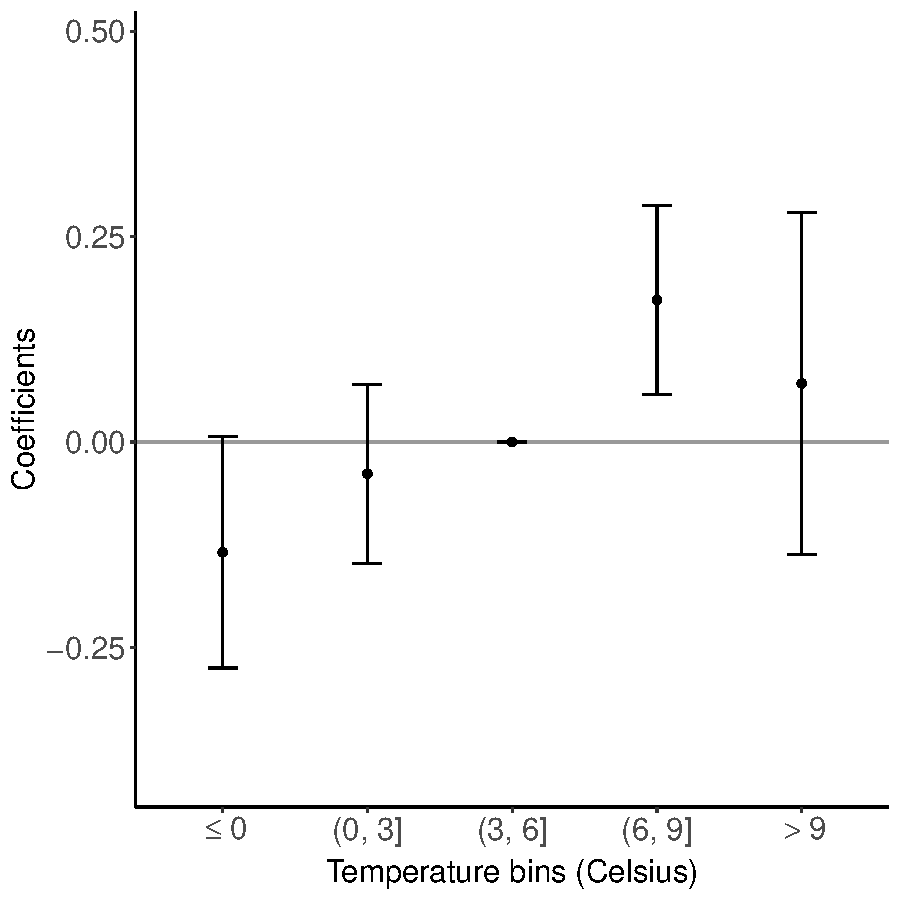
\includegraphics[width = \textwidth]{../Output/images/reg_major_2.pdf}
      \end{figure}
    \end{minipage}
    \begin{minipage}{0.43\textwidth}
      \begin{center}
        Science \\
        {\small (mean: 2.09 \%, median: 0.76 \%)}
      \end{center}
      \begin{figure}[h]
        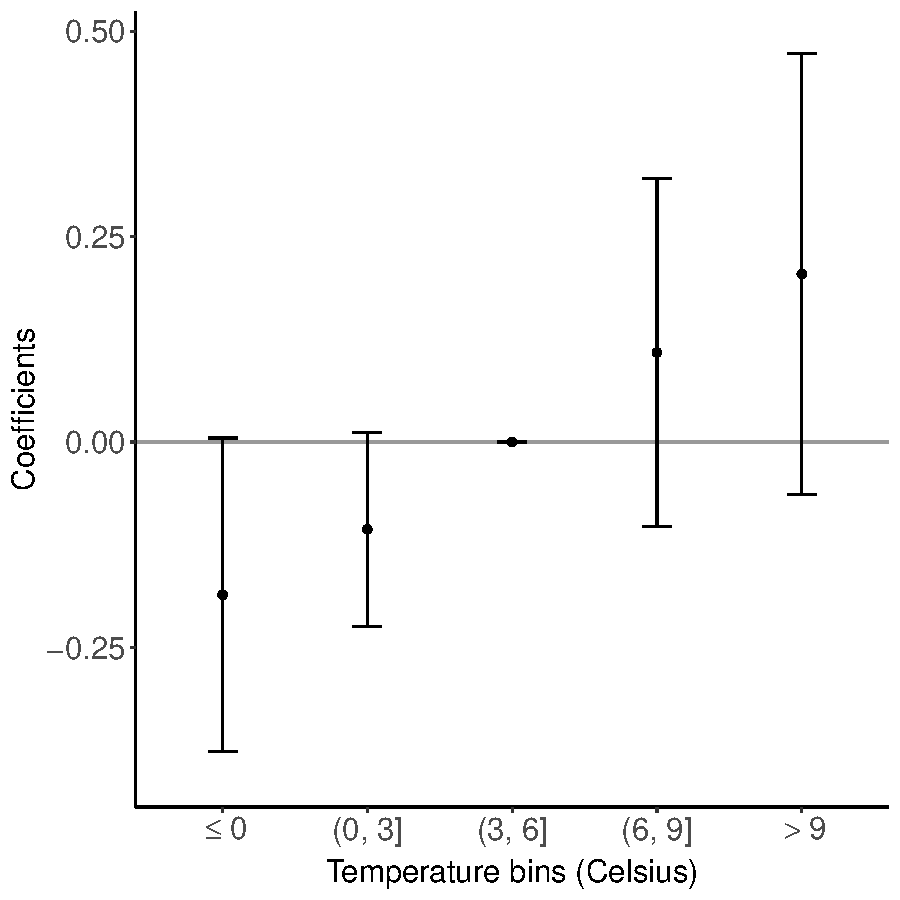
\includegraphics[width = \textwidth]{../Output/images/reg_major_4.pdf}
        \centering
      \end{figure}
    \end{minipage}
    \tiny
    \begin{tablenotes}
    \item Notes;
      The figures show the regression coefficients of the matriculation shares for UTokyo (\%) on temperature bins.
      In the left figure, the outcome is the matriculation share to humanity major from each prefecture.
      In the right figure, the outcome is the matriculation share to science major from each prefecture.
      Rainfall and cumulated snow on the ground (both on the exam days and average for 10 days before the exam) are included in the regression.
      The 90\% confidence intervals are shown.
      Prefecture fixed effects and year fixed effects are also included.
      Standard errors are clustered at the prefecture level.
    \end{tablenotes}
  \end{figure}
\end{frame}

\begin{frame}
  \frametitle{Conclusion}
  \begin{itemize}
    \item Weather on the exam date affects the matriculations for UTokyo
      \begin{itemize}
        \item A decrease in temperature from 3-6 \degree C to $<$0 \degree C decreases the probability of matriculation by 0.18 percentage points \\
          (9\% of the average and 22\% of the median matriculation shares)
        \item Snow on the ground cumulated more than 10cm decreases the probability of matriculation by 0.11 percentage points \\
          (5\% of the average and 13\% of the median matriculation shares)
      \end{itemize}
    \item Suggests that exam performance is negatively affected by winter weather
      \begin{itemize}
        \item Low temperature in the morning or during the exam negatively affects cognitive ability?
        \item Snow on the ground makes feet wet, which further decreases body temperature?
        \item Cumulated snow increases the risk of transportation delays?
      \end{itemize}
    \item Implications for university admissions process:
      \begin{itemize}
        \item Use other information such as extracurricular activities and personal statements for university admission?
        \item Adjust weights for Center Test and the second-stage exam?
      \end{itemize}
  \end{itemize}
\end{frame}

\appendix

\begin{frame}\frametitle{Temperature variations in each prefecture}
  \label{temp_dev_1}
  \begin{center}
    \begin{figure}
      %\caption{Map of matriculation shares (\%)}
      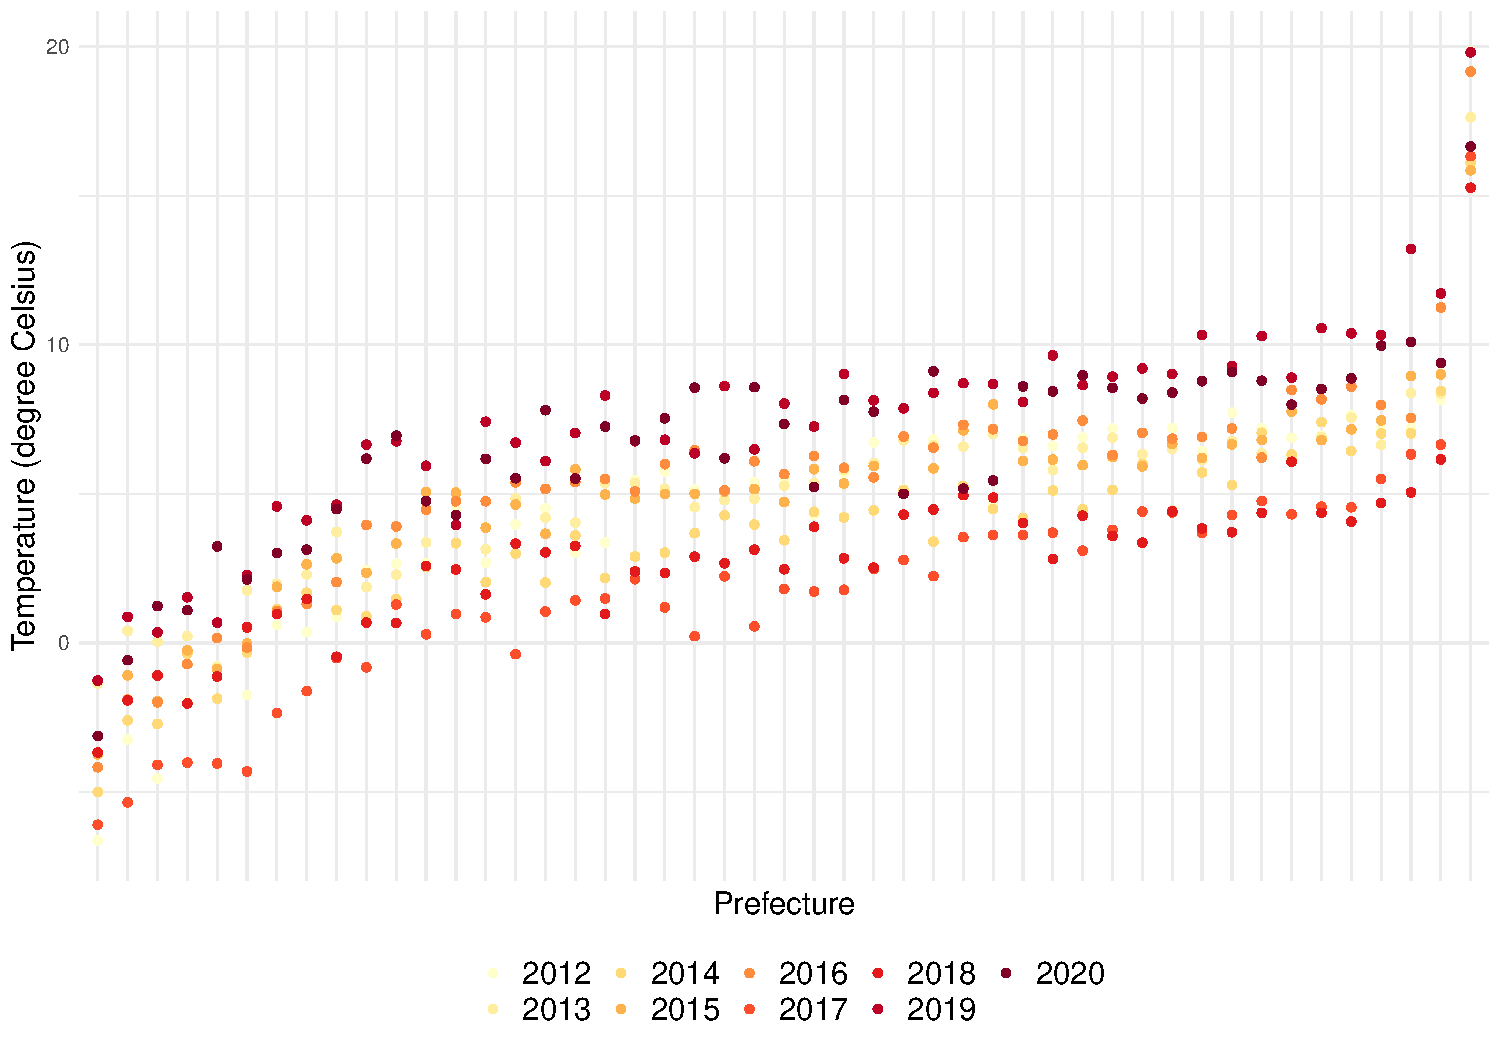
\includegraphics[width=9.5cm]{../Output/images/temperature_diff.pdf}
      \tiny
      \begin{tablenotes}
      \item Notes:
        Temperature at prefecture capitals between 6 AM and 6 PM on days of Center Test is used.
        Average across two test days in each year is shown in the figure.
        The prefectures are ordered by the mean temperature across years (lowest to left and highest to right).
      \end{tablenotes}
    \end{figure}
  \end{center}
  \hyperlink{est_eq}{\beamergotobutton{Estimation equation}}
\end{frame}

\begin{frame}\frametitle{Deviation of temperatures from within-prefecture averages \\ {\small Large variation in deviation of temperatures even within each year}} 
  \label{temp_dev_2}
  \begin{center}
    \begin{figure}
      %\caption{Map of matriculation shares (\%)}
      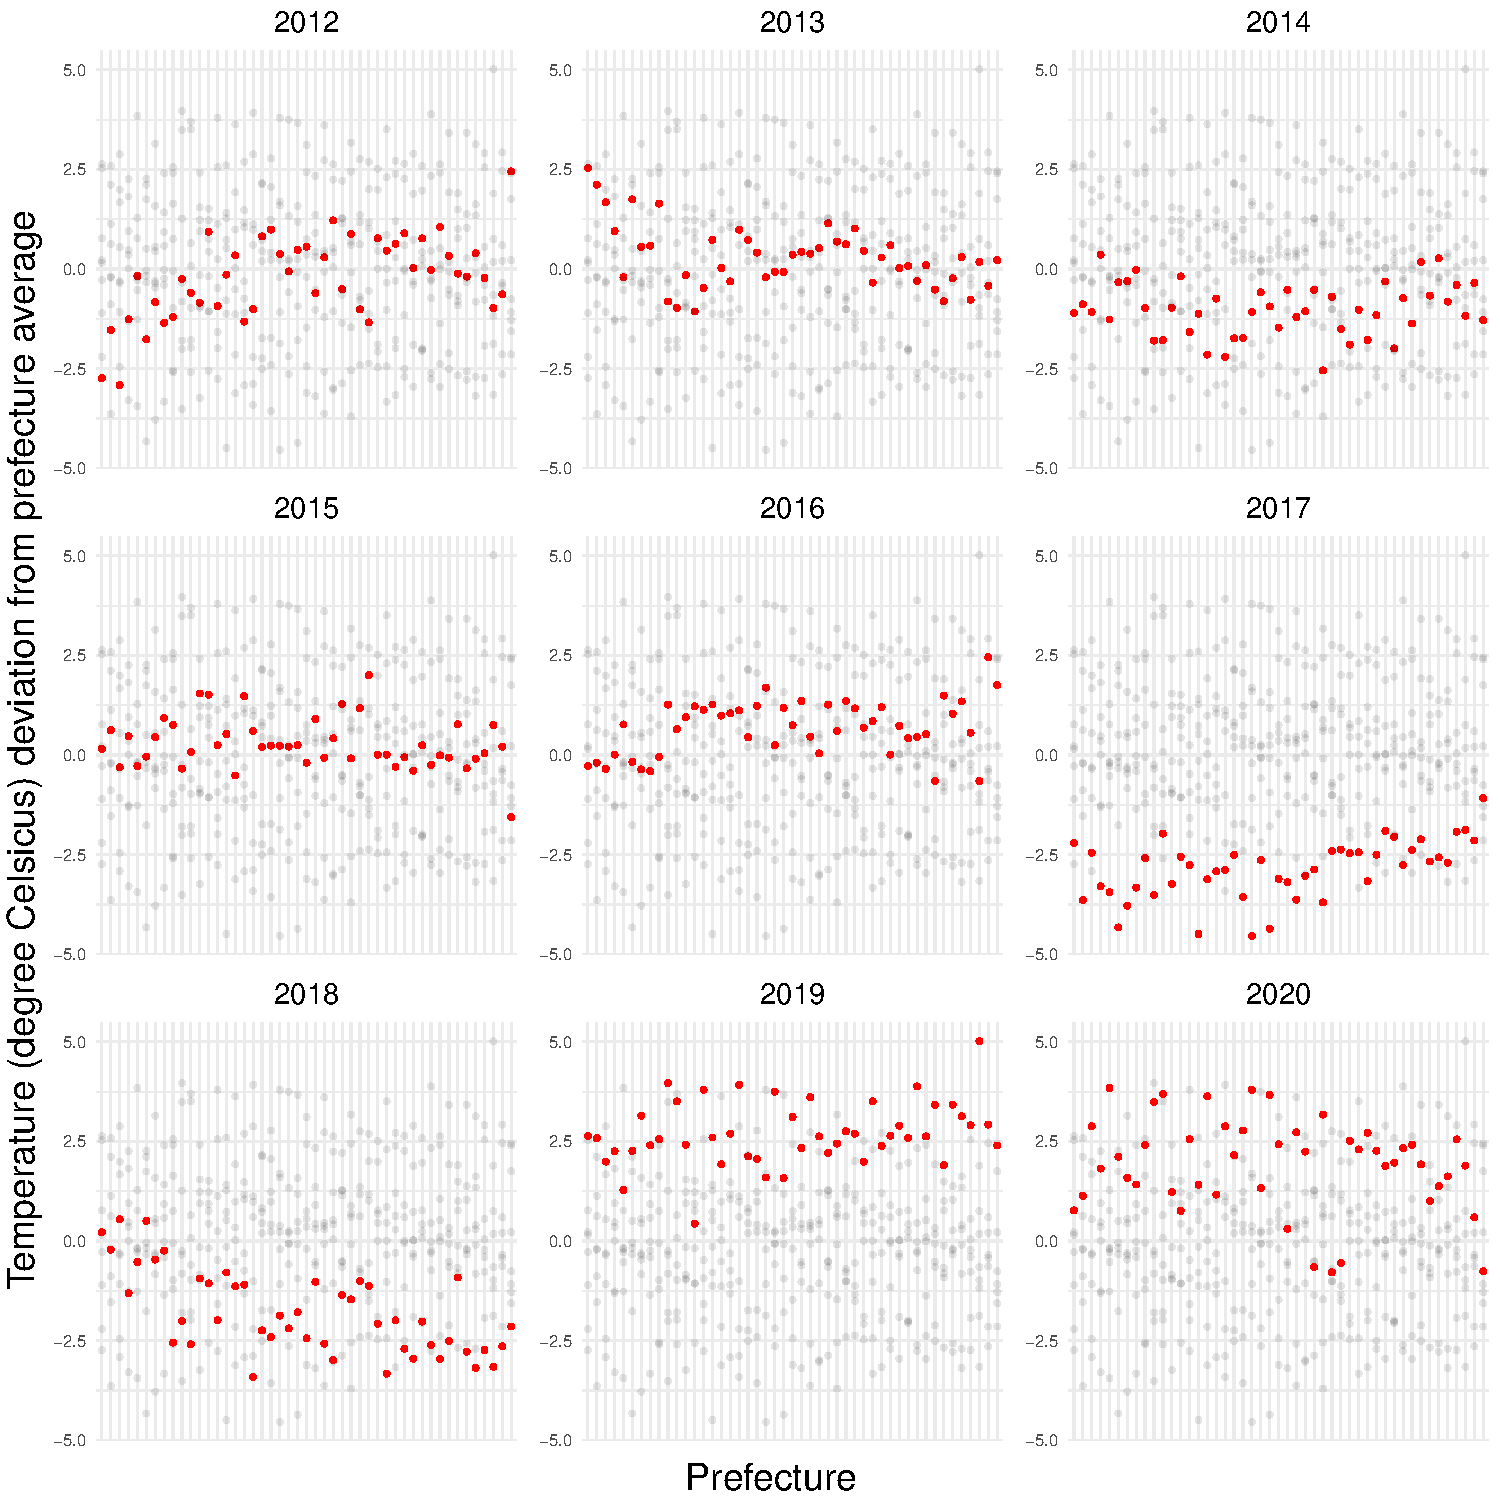
\includegraphics[width=6.2cm]{../Output/images/temperature_diff_by_year.pdf}
      \tiny
      \begin{tablenotes}
      \item Notes:
        Temperature at prefecture capitals between 6 AM and 6 PM on days of Center Test is used.
        Deviations of average temperatures across two test days from their within-prefecture means are shown in the figure by year.
        In each panel, red dots are the deviations in the year shown above and gray dots are the deviations in the other years.
        The prefectures are ordered by the mean temperature across years (lowest to left and highest to right). \\
      \item 
        \hyperlink{est_eq}{\beamergotobutton{Estimation equation}}
      \end{tablenotes}
    \end{figure}
  \end{center}
\end{frame}

\begin{frame}\frametitle{{\normalsize Effects of other weather variables on the matriculation shares (\%)} \\ {\small Cumulated snow on the exam date, not before exams, matters}}
  \begin{table}[h]
    \Wider[4em]{
    \center
    \fontsize{7}{5}\selectfont
    
% Table created by stargazer v.5.2.3 by Marek Hlavac, Social Policy Institute. E-mail: marek.hlavac at gmail.com
% Date and time: Wed, Oct 25, 2023 - 20:16:19
\begin{tabular}{@{\extracolsep{5pt}}lcccc} 
\\[-1.8ex]\hline 
\hline \\[-1.8ex] 
 & \multicolumn{4}{c}{\textit{Dependent variable:}} \\ 
\cline{2-5} 
\\[-1.8ex] & \multicolumn{4}{c}{Matriculation share (\%)} \\ 
\\[-1.8ex] & (1) & (2) & (3) & (4)\\ 
\hline \\[-1.8ex] 
 Rainfall (mm) (exam dates) &  &  & $-$0.02 & 0.06 \\ 
  &  &  & (0.10) & (0.08) \\ 
  & & & & \\ 
 Snowfall (cm) (exam dates) &  &  & 0.12 &  \\ 
  &  &  & (0.10) &  \\ 
  & & & & \\ 
 Cumulated snow (cm) (exam dates) &  &  &  & $-$0.002$^{*}$ \\ 
  &  &  &  & (0.001) \\ 
  & & & & \\ 
 Rainfall (mm) (previous 10 days) & $-$0.003 & $-$0.01 & $-$0.003 & $-$0.004 \\ 
  & (0.01) & (0.01) & (0.01) & (0.01) \\ 
  & & & & \\ 
 Snowfall (cm) (previous 10 days) & $-$0.02$^{*}$ &  & $-$0.02 &  \\ 
  & (0.01) &  & (0.01) &  \\ 
  & & & & \\ 
 Cumulated snow (cm) (previous 10 days) &  & $-$0.002$^{*}$ &  & 0.001 \\ 
  &  & (0.001) &  & (0.002) \\ 
  & & & & \\ 
\hline \\[-1.8ex] 
Temperature bins & Yes & Yes & Yes & Yes \\ 
Prefecture FE & Yes & Yes & Yes & Yes \\ 
Year FE & Yes & Yes & Yes & Yes \\ 
Observations & 423 & 423 & 423 & 423 \\ 
\hline 
\hline \\[-1.8ex] 
\textit{Note:}  & \multicolumn{4}{r}{$^{*}$p$<$0.1; $^{**}$p$<$0.05; $^{***}$p$<$0.01} \\ 
\end{tabular} 

    \tiny
    \begin{tablenotes}
    \item 
      The outcome variable is the matriculation shares (\%) for the University of Tokyo from each prefecture.
      The matriculation share is calculated based on the ratio of the number of students from high schools in the prefecture to the total number of matriculation.
      Standard errors are clustered at the prefecture level.
    \end{tablenotes}
  }
  \end{table}
\end{frame}


\end{document}

